% For LaTeX-Box: root = stat105_F15_exam1B.tex 
%%%%%%%%%%%%%%%%%%%%%%%%%%%%%%%%%%%%%%%%%%%%%%%%%%%%%%%%%%%%%%%%%%%%%%%%%%%%%%%%
%  File Name: stat105_F15_exam1B.tex
%  Purpose:
%
%  Creation Date: 24-09-2015
%  Last Modified: Tue Dec 15 02:31:56 2015
%  Created By:
%%%%%%%%%%%%%%%%%%%%%%%%%%%%%%%%%%%%%%%%%%%%%%%%%%%%%%%%%%%%%%%%%%%%%%%%%%%%%%%%
\documentclass[addpoints]{examsetup}\usepackage[]{graphicx}\usepackage[]{color}
%% maxwidth is the original width if it is less than linewidth
%% otherwise use linewidth (to make sure the graphics do not exceed the margin)
\makeatletter
\def\maxwidth{ %
  \ifdim\Gin@nat@width>\linewidth
    \linewidth
  \else
    \Gin@nat@width
  \fi
}
\makeatother

\definecolor{fgcolor}{rgb}{0.345, 0.345, 0.345}
\newcommand{\hlnum}[1]{\textcolor[rgb]{0.686,0.059,0.569}{#1}}%
\newcommand{\hlstr}[1]{\textcolor[rgb]{0.192,0.494,0.8}{#1}}%
\newcommand{\hlcom}[1]{\textcolor[rgb]{0.678,0.584,0.686}{\textit{#1}}}%
\newcommand{\hlopt}[1]{\textcolor[rgb]{0,0,0}{#1}}%
\newcommand{\hlstd}[1]{\textcolor[rgb]{0.345,0.345,0.345}{#1}}%
\newcommand{\hlkwa}[1]{\textcolor[rgb]{0.161,0.373,0.58}{\textbf{#1}}}%
\newcommand{\hlkwb}[1]{\textcolor[rgb]{0.69,0.353,0.396}{#1}}%
\newcommand{\hlkwc}[1]{\textcolor[rgb]{0.333,0.667,0.333}{#1}}%
\newcommand{\hlkwd}[1]{\textcolor[rgb]{0.737,0.353,0.396}{\textbf{#1}}}%

\usepackage{framed}
\makeatletter
\newenvironment{kframe}{%
 \def\at@end@of@kframe{}%
 \ifinner\ifhmode%
  \def\at@end@of@kframe{\end{minipage}}%
  \begin{minipage}{\columnwidth}%
 \fi\fi%
 \def\FrameCommand##1{\hskip\@totalleftmargin \hskip-\fboxsep
 \colorbox{shadecolor}{##1}\hskip-\fboxsep
     % There is no \\@totalrightmargin, so:
     \hskip-\linewidth \hskip-\@totalleftmargin \hskip\columnwidth}%
 \MakeFramed {\advance\hsize-\width
   \@totalleftmargin\z@ \linewidth\hsize
   \@setminipage}}%
 {\par\unskip\endMakeFramed%
 \at@end@of@kframe}
\makeatother

\definecolor{shadecolor}{rgb}{.97, .97, .97}
\definecolor{messagecolor}{rgb}{0, 0, 0}
\definecolor{warningcolor}{rgb}{1, 0, 1}
\definecolor{errorcolor}{rgb}{1, 0, 0}
\newenvironment{knitrout}{}{} % an empty environment to be redefined in TeX

\usepackage{alltt}

\usepackage{etoolbox}
\usepackage{tikz,pgfplots}
\usepackage{graphicx, fancyhdr}
\usepackage{amsmath, amsfonts}
\usepackage{color}

%% For LaTeX-Box: root = stat105_exam1_info.tex 
%%%%%%%%%%%%%%%%%%%%%%%%%%%%%%%%%%%%%%%%%%%%%%%%%%%%%%%%%%%%%%%%%%%%%%%%%%%%%%%%
%  File Name: stat105_exam1_info.tex
%  Purpose:
%
%  Creation Date: 24-09-2015
%  Last Modified: Thu Sep 24 13:51:36 2015
%  Created By:
%%%%%%%%%%%%%%%%%%%%%%%%%%%%%%%%%%%%%%%%%%%%%%%%%%%%%%%%%%%%%%%%%%%%%%%%%%%%%%%%
\newcommand{\course}[1]{\ifstrempty{#1}{STAT 105}{STAT 105, Section #1}}
\newcommand{\sectionNumber}{B}
\newcommand{\examDate}{October 1, 2015}
\newcommand{\semester}{FALL 2015}
\newcommand{\examNumber}{II}

\newcommand{\examTitle}{Exam \examNumber}

\runningheader{\course{\sectionNumber}}{Exam \examNumber}{\examDate}
\runningfooter{}{}{Page \thepage of \numpages}

\newcommand{\examCoverPage}{
   \begin{coverpages}
   \centering
   {\bfseries\scshape\Huge Exam I \par}
   \vspace{1cm}
   {\bfseries\scshape\LARGE \course{\sectionNumber} \par}
   {\bfseries\scshape\LARGE \semester \par}

   \vspace{2cm}

   \fbox{\fbox{\parbox{5.5in}{\centering 

      \vspace{.25cm} 
      
      {\bfseries\Large Instructions} \\

      \vspace{.5cm} 

      \begin{itemize}
         \item  The exam is scheduled for 80 minutes, from 8:00 to 9:20 AM. At 9:20 AM the exam will end.\\
         \item  A forumula sheet is attached to the end of the exam. Feel free to tear it off.\\
         \item  You may use a calculator during this exam.\\
         \item  Answer the questions in the space provided. If you run out of room, continue on the back of the page. \\
         \item  If you have any questions about, or need clarification on the meaning of an item on this exam, please ask your instructor. No other form of external help is permitted attempting to receive help or provide help to others will be considered cheating.\\
         \item  {\bfseries Do not cheat on this exam.} Academic integrity demands an honest and fair testing environment. Cheating will not be tolerated and will result in an immediate score of 0 on the exam and an incident report will be submitted to the dean's office.\\
      \end{itemize}

   }}}

   \vspace{2cm}

   \makebox[0.6\textwidth]{Name:\enspace\hrulefill}

   \vspace{1cm}

   \makebox[0.6\textwidth]{Student ID:\enspace\hrulefill}
   \end{coverpages}

}


\newcommand{\course}[1]{\ifstrempty{#1}{STAT 105}{STAT 105, Section #1}}
\newcommand{\sectionNumber}{B}
\newcommand{\examDate}{November 5, 2015}
\newcommand{\semester}{FALL 2015}
\newcommand{\examNumber}{III}

%%%%%%%%%%%%%%%%%%%%%%%%%%%%%%%%%%%%%%%%%%%%%%%%%%%%%%%%%%%%%%%%%%%%%%%%%%%%%%%%
\IfFileExists{upquote.sty}{\usepackage{upquote}}{}
\begin{document}

%-- : R code (Code in Document)



\examCoverPage

\begin{questions}

\question[2]
(TRUE/FALSE) A random sample of 1000 student's Statistics exam scores was drawn from the population of all possible Stat scores (an unknown distribution).
Once the sample mean is computed, it can be viewed as the distribution/population mean.

\vspace{1cm}

\question[2]
(TRUE/FALSE) While trying to figure out the probability that the sample mean for a data of size 10 would exceed a value, we can apply the central limit theorem.

\vspace{1cm}

% \question
%
% %-- question1: R code (Code in Document)
% <<question1, echo=FALSE, cache=TRUE, include = TRUE>>=
%    set.seed(10012015.1)
% 
%    #precision vs accuracy
%    high_pH <- round(rnorm(8,11.4,.1), 1)
%    low_pH <- round(rnorm(8,3,.2), 1)
% @
% 
% A pH meter is a tool used to determine the acidity of a liquid. 
% Calibrating them requires the user to take repeated measurements of a liquid that has a known pH and adjust the meter's measurements to match.
% Below are measurements on two different liquids, one with a known pH of 3 and the other with a known pH of 11.
% 
% \begin{itemize}
% 
%    \item Readings with pH = 11: $ paste(high_pH,collapse=", ") $ \\
% 
%    \item Readings with pH = 3: $ paste(low_pH,collapse=", ") $ \\
% 
% \end{itemize}
% 
% 
% \begin{parts}
%    \part[2] At what pH is the meter more accurate?
% 
%    \vspace{1cm}
% 
%    \part[2] At what pH is the meter more precise?
% 
%    \vspace{1cm}
% 
% \end{parts}
% 
% \vspace{1cm}

\question 
%-- functionsAndDatasets: R code (Code in Document)

A sample of size 3 was drawn from a population and the resulting observations are reported below. 
$$
   2.2, 2, 10.3
$$
Using these observed values, report the following:

\vspace{1cm}

\begin{parts}

   \part[2] the mean  
   \vspace{1.5cm}

   \part[2] the median
   \vspace{1.5cm}

   \part[2] the variance 
   \vspace{2cm}

   \part[2] the standard deviation 
   \vspace{1.5cm}

\end{parts}

\newpage

\question
An agriculturist is attempting to determine which of three species of corn (A, B, and C) yield the most grain per acre.
Since the yield may depend on the fertilizer used, the researcher intends to use fertilizers with different concentrations of Nitrogen as well - low Nitrogen, medium-low Nitrogen, medium-high Nitrogen, and high Nitrogen.
There are 8 fields (scattered around Iowa) available to perform this expiriment. 
Each field is divided into 24 single acre plots and the combinations of species and fertilizer are randomly assigned so that within each field every combination is used exactly twice.
At harvest time, the amount of grain each plot yields is recorded and the combination of corn species and fertilizer that gives the highest average yield is chosen.

\begin{parts}
   \part[2] Is this an experiment or an observational study? Explain.

  \vspace{2cm}

   \part Identify the following (if there was not one, simply put "not used"). Additionally, label each as continuous or discrete.

  \vspace{1cm}

   \begin{subparts}
      \subpart[2] Response variable(s):

      \vspace{2cm}

      \subpart[2] Experimental variable(s):

      \vspace{2cm}

      \subpart[2] Blocking variable(s):

      \vspace{2cm}

   \end{subparts}


   \part[2] Was replication used in this study? If so, where was it applied? If not, how could we have applied it?

  \vspace{2cm}

\end{parts}

\pagebreak

\question 

%-- : R code (Code in Document)


A company specializing in the installation and maintanence of ``infinity pools" records the number of service requests they receive each month for two years.
The number of requests are presented in the table below:

%-- : R code (Code in Document)
\begin{knitrout}
\definecolor{shadecolor}{rgb}{0.969, 0.969, 0.969}\color{fgcolor}\begin{kframe}
\begin{verbatim}

  The decimal point is 1 digit(s) to the right of the |

  0 | 122333444
  0 | 556669999
  1 | 4
  1 | 77
  2 | 013
\end{verbatim}
\end{kframe}
\end{knitrout}

Note that \verb!0 | 4! represents 4 and \verb!1 | 2! represents 12. 
In this case, the first quartile is $Q(.25) = 3.5$, 
the median is 6, and the third quartile is $Q(.75) = 11.5$.

\begin{parts}

  \part[10] Using the axes below, create a box plot to summarize the data. Label all important values. Draw a star over unusual observations.

  \vspace{2cm}

%-- : R plot (results in document)
\begin{knitrout}
\definecolor{shadecolor}{rgb}{0.969, 0.969, 0.969}\color{fgcolor}
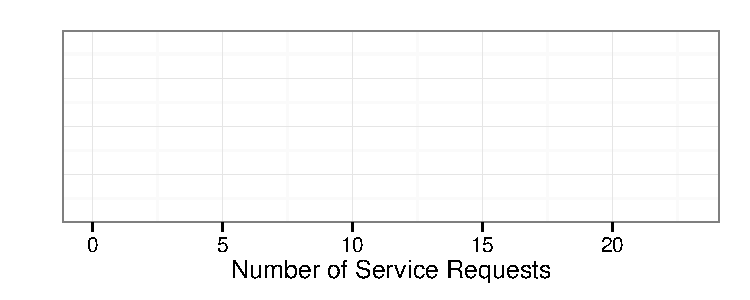
\includegraphics[width=.9\linewidth]{figure/unnamed-chunk-4-1} 

\end{knitrout}

  \vspace{2cm}

%    \part[4] 
%    The distance driven by the company's maintanence workers to each service call were also recorded. 
%    A theorhetical Q-Q plot comparing the distances to the quantiles of a normal distribution is presented below.
%    The line represents where the normal quantiles and driving distance quantiles would match perfectly.
%    What does this graph tell us about the distribution of the distance that workers drive?
%  
%  %-- : R code (Code in Document)
%  <<echo=FALSE, cache=FALSE, include = TRUE>>=
%  
%     drives <- round(rgamma(sum(samp), 4, .125),1)
%  
%  @
%  
%  \begin{center}
%     
%  %-- : R plot (results in document)
%  <<fig.width=4, fig.height=4, out.width='.5\\linewidth', echo=FALSE>>=
%  
%     qqplot.data <- function (vec) # argument: vector of numbers
%     {
%          # following four lines from base R's qqline()
%          y <- quantile(vec[!is.na(vec)], c(0.25, 0.75))
%       x <- qnorm(c(0.25, 0.75))
%         slope <- diff(y)/diff(x)
%         int <- y[1L] - slope * x[1L]
%  
%           d <- data.frame(resids = vec)
%  
%           ggplot(d, aes(sample = resids)) + stat_qq() + geom_abline(slope = slope, intercept = int, color = "red") + theme_bw() + xlab("Theorhetical quantiles") + ylab("Distance Driven")
%  
%     }
%     qqplot.data(drives)
%  @
%  \end{center}

\end{parts}
\pagebreak

\question

%-- : R code (Code in Document)



A survey given to members of a national engineering honor society who have recently graduated is attempting to determine the relationship between salary and GPA.
The graph below displays 150 responses.

The results are depicted below (using GPA on the x-axis):
\begin{center}
\begin{knitrout}
\definecolor{shadecolor}{rgb}{0.969, 0.969, 0.969}\color{fgcolor}
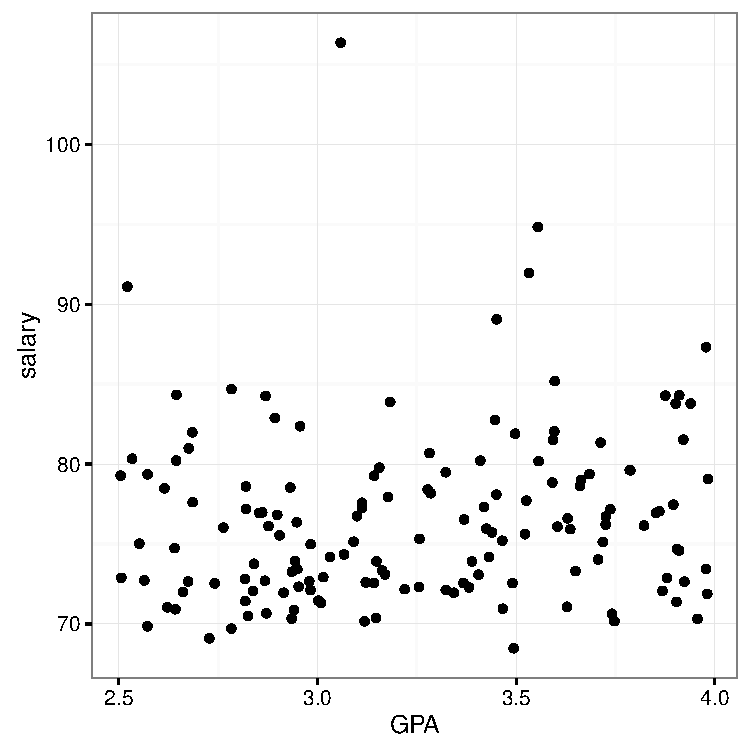
\includegraphics[width=.5\linewidth]{figure/unnamed-chunk-6-1} 

\end{knitrout}
\end{center}

Here are some summaries of the data (again using the actual score as the x-value and the person's evaluation of their score as the y-value):

$$
   \sum_{i=1}^{150} x_i = 487 \hspace{3cm} \sum_{i=1}^{150} x_i^2 = 1609 \\
$$

$$
   \sum_{i=1}^{150} y_i = 11474 \hspace{3cm} \sum_{i=1}^{150} y_i^2 = 882126 \\
$$

$$
   \sum_{i=1}^{150} x_i y_i = 37299
$$

\begin{parts}
   \part Using the summaries above, the survey workers fit a linear relationship between \textbf{GPA} (x) and \textbf{salary} (y). 
   \begin{subparts}
      \subpart[5] Write the equation of the fitted linear relationship. 
      \vspace{2cm}
      \subpart[5] Using the fitted line, what do we suppose the salary will be for an engineer with a GPA of 3.0?
      \vspace{2cm}
   \end{subparts}

   \newpage 

   \part 
   Discouraged by the relationship between salary and GPA, the surveyors remember that they know the address of each respondant and are able to determine the median income of the area in which the respondant lives. 
   The JMP output below comes from fitting a linear relationship using the annual salary of the respondant (``\verb!salary!") and the median income of the area in which the respondant lives (\verb!med_salary_loc!).

   \centerline{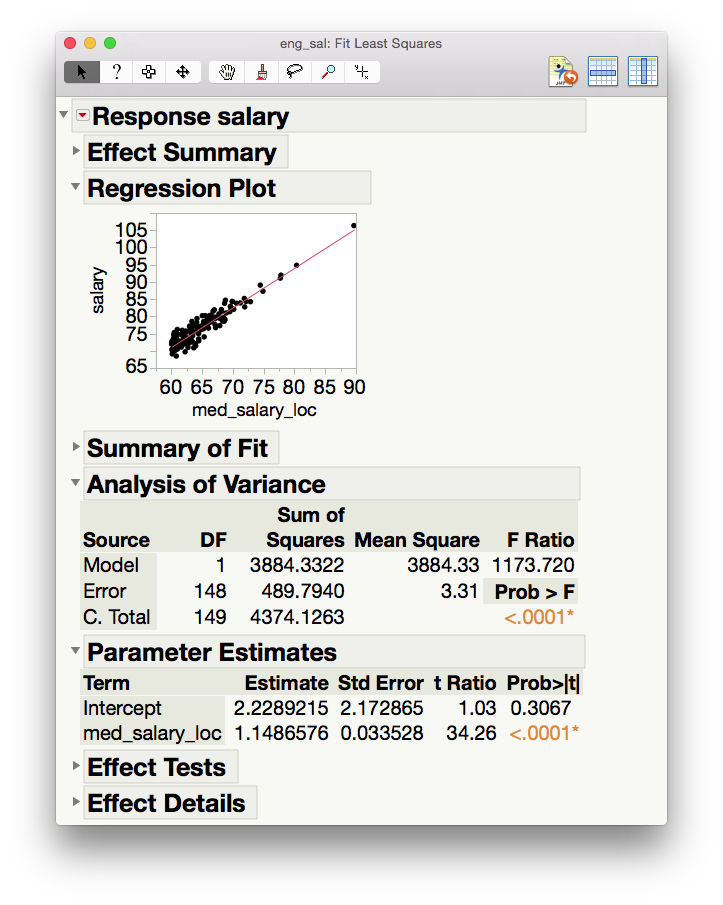
\includegraphics[scale=.4]{fit_sal}}

   \begin{subparts}
      \subpart[5] Write the equation of the fitted linear relationship.
      \vspace{2cm}
      \subpart[5] Find and interpret the value of $R^2$ for the fitted quadratic relationship.
      \vspace{2cm}
   \end{subparts}
\end{parts}

\question
A winery is experimenting with blending a small amount of non-grape tastes into its current harvest of grapes (to add ``notes").
They are considering three fruit additions (apple, cherry, and kiwi) and two spice additions (oak and vanilla).
Three wine experts working for the company test the fruit/spice combinations and provide a rating from 0 to 10 (with 10 being the highest).

The results are recorded below.

%-- : R code (Code in Document)


\begin{table}[h]
\centering
\begin{tabular}{lrr}
   & \multicolumn{2}{c}{Spice} \\
\cline{2-3}
Fruit & Oak & Vanilla \\ \hline \hline
Apple   & 9.8 & 8.4 \\
        & 9.9 & 8.9 \\
        & 9.3 & 8.3 \\
Cherry  & 8.3 & 5.3 \\
        & 5.5 & 4.9 \\
        & 5.7 & 4.7 \\
Kiwi    & 8 & 7 \\
        & 8.1 & 7.3 \\
        & 7.6 & 6.6 \\
\hline
\end{tabular}
\end{table}

The following summaries may help in this problem:

%-- : R code (Code in Document)


\begin{table}[h]
\centering
\begin{tabular}{lrrr}
   & \multicolumn{2}{c}{Spice} \\
\cline{2-3}
Fruit & Oak & Vanilla \\ \cline{1-3}\cline{1-3}
Apple    & $\bar{y}_{11}$ = 9.67 & $\bar{y}_{12}$ = 8.53 & $\bar{y}_{1 \cdot}$ = 9.1 \\
Cherry   &                                                                                                     & $\bar{y}_{2 \cdot}$ = 5.04 \\
Kiwi     & $\bar{y}_{31}$ = 7.9 & $\bar{y}_{32}$ = 6.97 & $\bar{y}_{3 \cdot}$ = 7.44 \\
\cline{1-3}
         & $\bar{y}_{\cdot 1}$ = 7.69 &                                                                       & $\bar{y}_{\cdot \cdot}$ = 7.19 \\
\end{tabular}
\end{table}


\begin{parts}

   \part[2] Report the value of $\bar{y}_{21}$
   \vspace{2cm}

   \part[2] Report the value of $\bar{y}_{\cdot 2}$
   \vspace{2cm}

   \part[3] Find the fitted main effect of fruit, $a_1$, $a_2$, and $a_3$, that you would get from factorial model that ignores interactions.
   \vspace{3cm}

   \part[3] Ignoring possible interactions, give the estimated values $\hat{y}_{22}$ and $\hat{y}_{23}$.
   \vspace{3cm}

   \part[2] How do the estimated values computed above compare to the average for the same combinations seen in the data? 
            Does it appear that ignoring interactions was a good choice?
   \vspace{2cm}

   \part[5] Using the template below, create a profile plot for this data:

%-- : R plot (results in document)
\begin{knitrout}
\definecolor{shadecolor}{rgb}{0.969, 0.969, 0.969}\color{fgcolor}

{\centering 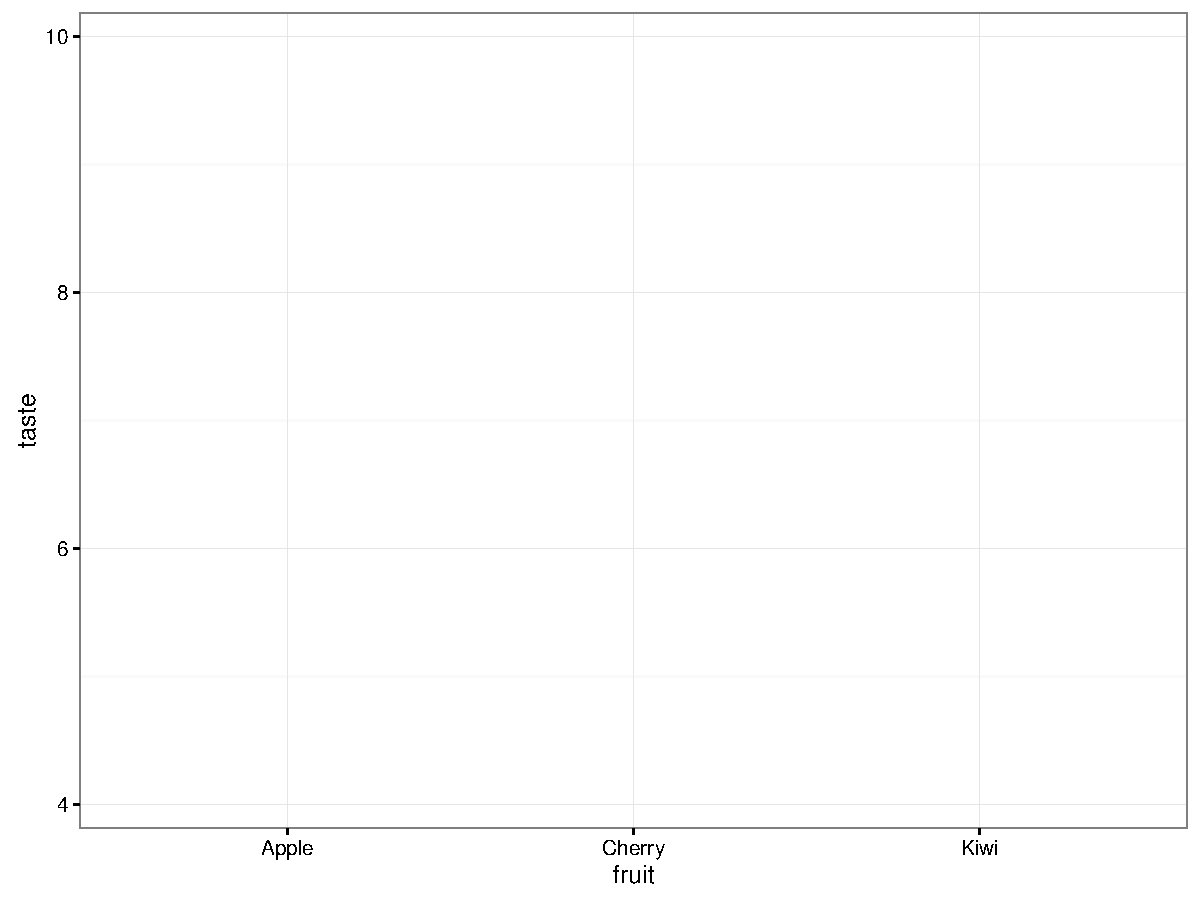
\includegraphics[width=.7\linewidth]{figure/unnamed-chunk-9-1} 

}



\end{knitrout}

   \part[2] Using the plot does it appear that there are interactions between fruit and spice type? Which combination would you recommend?
   \vspace{2cm}
\end{parts}

\newpage

\question

Let $X$ be a normal random variable with a mean of 1 and a varaince of 16 (i.e., $X \sim N(1,16)$) and let $Z$ be a random variable following a standard normal distribution.
Find the following probabilities (note: the attached standard normal probability table may be helpful):
\begin{parts}
     \part[2] $P(Z \le 1)$

     \vspace{2cm}

     \part[2] $P(|Z| \ge 2)$

     \vspace{2cm}

     \part[2] $P(0 \le X < 5)$

     \vspace{2cm}

     \part[2] $P(|X| \le 5)$

     \vspace{2cm}

\end{parts}

\question 

Suppose that $X$ is a continuous random variable with cumulative density function (cdf):
$$
F(x) = 
\begin{cases}
    0 &  x < 0 \\
   1 - e^{-3x} &  x \ge 0
\end{cases}
$$

\begin{parts}

\part[2] What is the probability that $X$ takes a value less than 1?

     \vspace{2cm}

\part[2] What is the probability that $X$ takes a value greater than 2?

     \vspace{2cm}

\part[2] Derive f(x), the probability density function.

     \vspace{2cm}

\end{parts}

\newpage

\question

Suppose we have a bag containing five tiles, three of which are labelled 1 and two of which are labelled 2.
Assume that each of the five tiles has an equal chance of being drawn.
The number on the tile tells us how many times we will roll a fair die.
For instance, if we draw a tile with the number 2 on it, we will roll a die twice but if we draw a tile with a 1 on it, we will only roll a die once.
For this problem, 
\begin{itemize}
   \item let $X$ be the number on the tile 
   \item let $Y$ be the sum of our rolls \\
\end{itemize}

\begin{parts}
   \part[2] Find $f_X(x)$.
   \vspace{2cm}
   \part[2] Find $f_{Y|X}(6|1)$.
   \vspace{2cm}
   \part[2] Find the joint probability $f(1,6)$.
   \vspace{2cm}
   \part[2] Find the joint probability $f(2,6)$.
   \vspace{2cm}
   \part[3] Find $f_{Y}(6)$.
   \vspace{2cm}
   \part[2] Find $f_{X|Y}(2|6)$.
   \vspace{2cm}
\end{parts}

\newpage

\question
O-rings are elastomer loops designed to create a seal between the interface of two parts of a mechanical device.
Because the elasticity of the material used to make them can be impacted by temperature (which can lead to the seal being broken) it is important to make sure that the O-ring is functional at the temperatures the part they are used in will be exposed to.
Two composites (Composite X and Composite Y) are being tested in an O-ring that will be used in a part of a satellite that will be exposed to very low temperatures.
A sample of 50 O-rings from each composite are placed in a chamber, where the temperature is gradually reduced until the seal is broken.
Suppose that each composite has some mean failure temperature, $\mu_X$ for Composite X and $\mu_Y$ for Composite Y, and some variance in failure temperature, 
$\sigma_X^2$ for Composite X and $\sigma_Y^2$ for Composite Y. 
Before any observations are recorded, we can consider the sampled values from Composite X to be random variables $X_1, X_2, \ldots, X_{50}$ with $\mathbb{E}(X_i) = \mu_X$ and $Var(X_i) = \sigma_X^2$.
We can also consider the sampled values from Composite Y to be random variables $Y_1, Y_2, \ldots, Y_{50}$ with $\mathbb{E}(Y_i) = \mu_Y$ and $Var(Y_i) = \sigma_Y^2$.

Let $\bar{X} = \frac{1}{50} X_1 + \frac{1}{50} X_2 + \ldots + \frac{1}{50} X_{50}$ and let $\bar{Y} = \frac{1}{50} Y_1 + \frac{1}{50} Y_2 + \ldots + \frac{1}{50} Y_{50}$.

\begin{parts}
   \part[3] What is the expected value of $\bar{X}$ (use appropriate symbols if needed).
   \vspace{2cm}
   \part[3] What is the variance of $\bar{X}$ (use appropriate symbols if needed).
   \vspace{2cm}
   \part[3] What is the distribution of $\bar{X}$ (use appropriate symbols if needed).
   \vspace{2cm}
   \part[3] What is the expected value of $\bar{Y}$ (use appropriate symbols if needed).
   \vspace{2cm}
   \part[3] What is the variance of $\bar{Y}$ (use appropriate symbols if needed).
   \vspace{2cm}
   \part[3] What is the distribution of $\bar{Y}$ (use appropriate symbols if needed).
   \vspace{2cm}
   \part[6] Let $\bar{D} = \bar{X} - \bar{Y}$. What is the distribution of $\bar{D}$ (use appropriate symbols if needed).
   \vspace{2cm}
\end{parts}

\question
   After running the O-ring experiment, the researchers found $\bar{x} = 50$ K and $\bar{y} = 53$ K. 
   Suppose that $\sigma_X^2 = 10$ and $\sigma_Y = 20$.
\begin{parts}
   \part[4] Provide a 90\% confidence interval for $\mu_X$.
   \vspace{3cm}
   \part[4] Provide a 99\% confidence interval for $\mu_X$.
   \vspace{3cm}
   \part[4] Provide a 95\% confidence interval for $\mu_Y$.
   \vspace{3cm}
   \part[6] Provide a 95\% confidence interval for $\mu_X - \mu_Y$ (hint: you can use the distribution of $\bar{D}$). Does this provide any evidence that one O-ring is better than the other?
   \vspace{3cm}
   \part[2] Is there any evidence that one O-ring is better than the other?
\end{parts}

\newpage

\question
   
   A company recently did a major overhaul to their server system hardware and is checking to make sure that there have been no changes in the download speed.
   The previous download speed had an average of 63.4 Mbps.
   A systems analyst took 10 readings on the download speeds during the course of a day to check. 
   Her results are below (in Mbps):

%-- : R code (Code in Document)


\begin{center}
   63.63, 63.4, 63.51, 63.14, 63.38, 63.35, 63.53, 63.37, 63.53, 63.71
\end{center}

The sample average is 63.45 and the sample variance is 0.026.

\begin{parts}
   

\part[5] Provide a 90\% confidence interval for the mean download speed.
\vspace{2cm}

\part[5] Provide a 95\% lower confidence bound for the mean download speed.
\vspace{2cm}

\part[10] Conduct a hypothesis test at the 95\% confidence level for the null hypothesis $\mu = 63.4$ against the alternative $\mu \ne 63.4$. Include your hypothesis statement, the test statistic, the p-value, your decision rule, and your conclusion.

\end{parts}
   

\end{questions}

\end{document}
